% !TEX root = MAIN.tex

%\chapter{FAQAS usage methodology}
\chapter{FAQAS Usage Methodology}
\label{chapter:methodology}

FAQAS led to the development of a toolset that includes the following components:
\begin{itemize}
\item MASS (Mutation Analysis for Space Software), a tool that automatically executes code-driven mutation analysis. Code-driven mutation analysis consists of automatically generating mutants by altering the source code of the software under test. MASS implements a pipeline that makes it feasible in the context of space software.
\item DAMAt (DAta-driven Mutation Analysis with Tables), a tool that automatically executes data-driven mutation analysis. Data-driven mutation analysis is an approach newly defined within FAQAS, which, instead of mutating the implementation of the software under test, alters the data exchanged by software components. Data-driven mutation analysis enables the injection of faults that affect simulated components (e.g., sensors), which is not feasible with traditional, code-driven mutation analysis.
\item SEMuS (Symbolic Execution-based MUtant analysis for Space software), a tool that automatically generates test inputs based on code-driven mutation analysis results.
\end{itemize}

\begin{figure}[tb]
\begin{center}
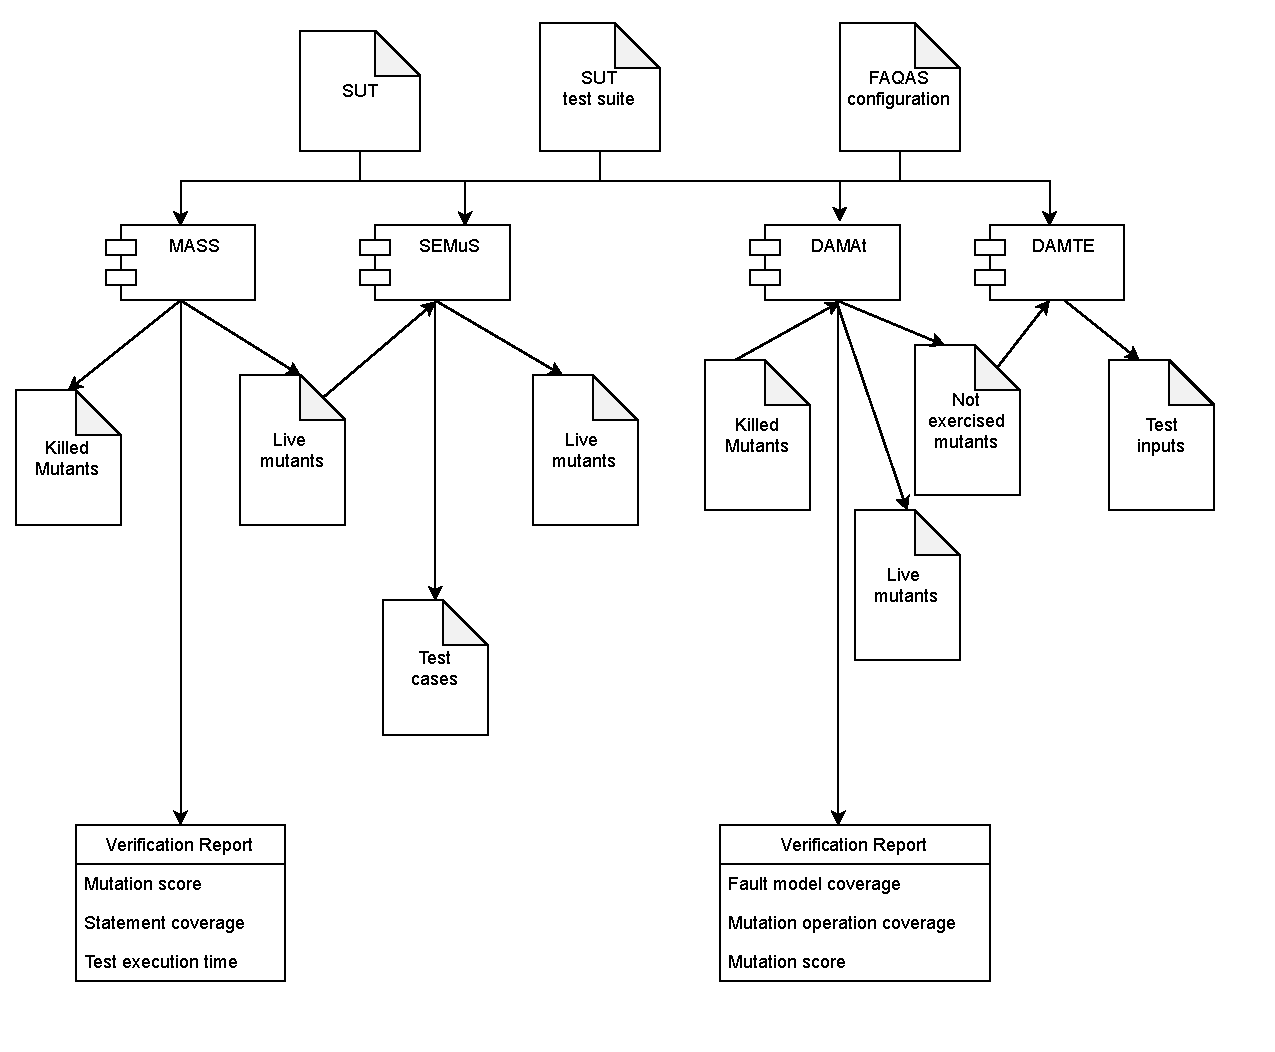
\includegraphics[width=0.8\textwidth]{images/FAQAS_drawio}
\caption{Overview of the FAQAS toolset}
\label{fig:FAQAS:toolset}
\end{center}
\end{figure}

The FAQAS activity also led to the definition and feasibility study of DAMTE, a methodology supported by the KLEE symbolic execution engine for the generation of test inputs based on data-driven mutation analysis results. However, DAMTE has shown to not be feasible in practice, with the current state-of-the-art test generation toolset.

Figure~\ref{fig:FAQAS:toolset} provides an overview of the input and outputs of the FAQAS toolset. All the components take as input the software under test (SUT), its test suite, and a set of configuration files.
MASS generates as output a set of live mutants (i.e., mutants that do not lead to a test suite failure), a set of killed mutants (i.e., mutants that lead to a test suite failure), and information useful to draft a verification report, which includes the statement coverage of the SUT test suite, the mutation score, and the execution time of test cases.
SEMuS takes as input the list of live mutants detected by MASS and aims to generate test cases that kill them. After the
 execution of SEMuS, engineers have a set of additional test cases to be integrated into the SUT test suite and a list of live mutants (i.e., mutants for which SEMuS was not able to identify test inputs killing them). Live mutants shall be manually inspected by engineers to either determine if they are equivalent mutants or to manually derive a test input killing them.
 DAMAt generates as output a set of killed mutants (i.e., mutants that, during testing, successfully alter the data, and lead to test case failures), a set of live mutants (i.e., mutants that, during testing, successfully alter the data, but do not lead to test case failures), and a set of not executed mutants (i.e., mutants that, during testing, could not alter any data because the data they target is never exercised by the SUT); also, it provides information useful to draft a verification report, which includes the fault model coverage, the mutation operation coverage, and the mutation score.
 DAMTE is a manual procedure supported by the KLEE toolset that enables an engineer to automatically derive inputs that increase the fault model coverage and the mutation operation coverage.

In the following, we describe how the results generated by the FAQAS toolset enable the assessment and improvement of a test suite.
We focus on the fully automated tools, that is, MASS, DAMAt, and SEMuS.


\section{Code-driven Mutation Analysis: MASS}
\label{sec:meth:mass}

Code-driven Mutation Analysis shall be performed by applying the MASS toolset following the setup procedures described in the SUM. Figure~\ref{fig:MASS} provides an overview of the MASS workflow as presented in Section~\ref{sec:approach}. In addition it provides additional blocks, draw with dotted lines, showing how the MASS output might be used to improve the test suite.
\STARTCHANGEDFINAL
The step \emph{Improve Test Suite} is a manual task that shall be performed by the engineers, however the \emph{Augmented SUT Test Suite} and \emph{Previously Live Mutants} outputs are created automatically by our methodology.
\ENDCHANGEDFINAL
Also, we added the step \EMPH{Configure MASS} (i.e., \emph{Step 0}) to show the main configuration choices to be made by the engineer before running mutation analysis.

To run MASS, at a high-level, the engineer needs to make the following choices
\begin{itemize}
\item \EMPH{Select the source files to mutate}. Generally, all the source files of the SUT shall be considered for mutation. If the test suite targets only a subset  of files, the engineer can focus on that subset.
\item \EMPH{Select the sampling strategy}. If the test suite of the SUT takes more than one hour to be executed, we suggest to rely on the \emph{FSCI} mutant sampling strategy. Otherwise, engineers can execute all the mutants (i.e., set \emph{sampling=NO})
\item \EMPH{Enable test suite reduction and prioritization}. This choice enables MASS to further reduce test execution time by executing only a portion of the selected test cases based on statement coverage (see Section~\ref{sec:approach}). In case of system test suites testing an SUT with multiple tasks running in parallel we suggest to avoid reducing the test suite.
\end{itemize}

\STARTCHANGEDFINAL
% !TEX root =  ../MAIN.tex

\begin{table}[tb]
\footnotesize
\centering
\caption{\MASS minimal set of parameters to be configured.}
\label{table:to_configure}
\begin{tabular}{llp{7.5cm}}
\hline
\textbf{Script Name}  & \textbf{Parameter} &  \textbf{Description} \\
\hline
mass\_conf.sh & BUILD\_SYSTEM &  Specifies the building system type.\\
& PROJ &  Path of the SUT root  directory.\\
& PROJ\_SRC &  Path of the SUT source directory.\\
& PROJ\_TST &  Path of the SUT test  directory.\\
& PROJ\_COV &  Path of the directory with SUT coverage information.\\
& PROJ\_BUILD &  Path of the directory where the compiled binary is stored.\\
& ORIGINAL\_MAKEFILE &  Path to the original build script.\\
& COMPILATION\_CMD &  Compilation command of the SUT.\\
\hline
PrepareSUT.sh & None &  Commands shall be provided manually.\\
\hline
mutation\_additional\_functions.sh & run\_tst\_case  &  Implementation of the Bash function run\_tst\_case that executes the test case passed as a parameter.\\
\hline
\end{tabular}
\end{table}

In a nutshell the minimal set of parameters to be configured for MASS are listed and described in Table~\ref{table:to_configure}. Particularly, the SUT engineer shall specify: the building system type, the SUT paths (e.g., source code, test suite directory, code coverage directory, build script), the SUT compilation commands, and commands for executing a single test case of the test suite.
\ENDCHANGEDFINAL

For the other configuration choices for MASS, the default options are generally appropriate for most of the SUTs.

\begin{figure}[tb]
\begin{center}
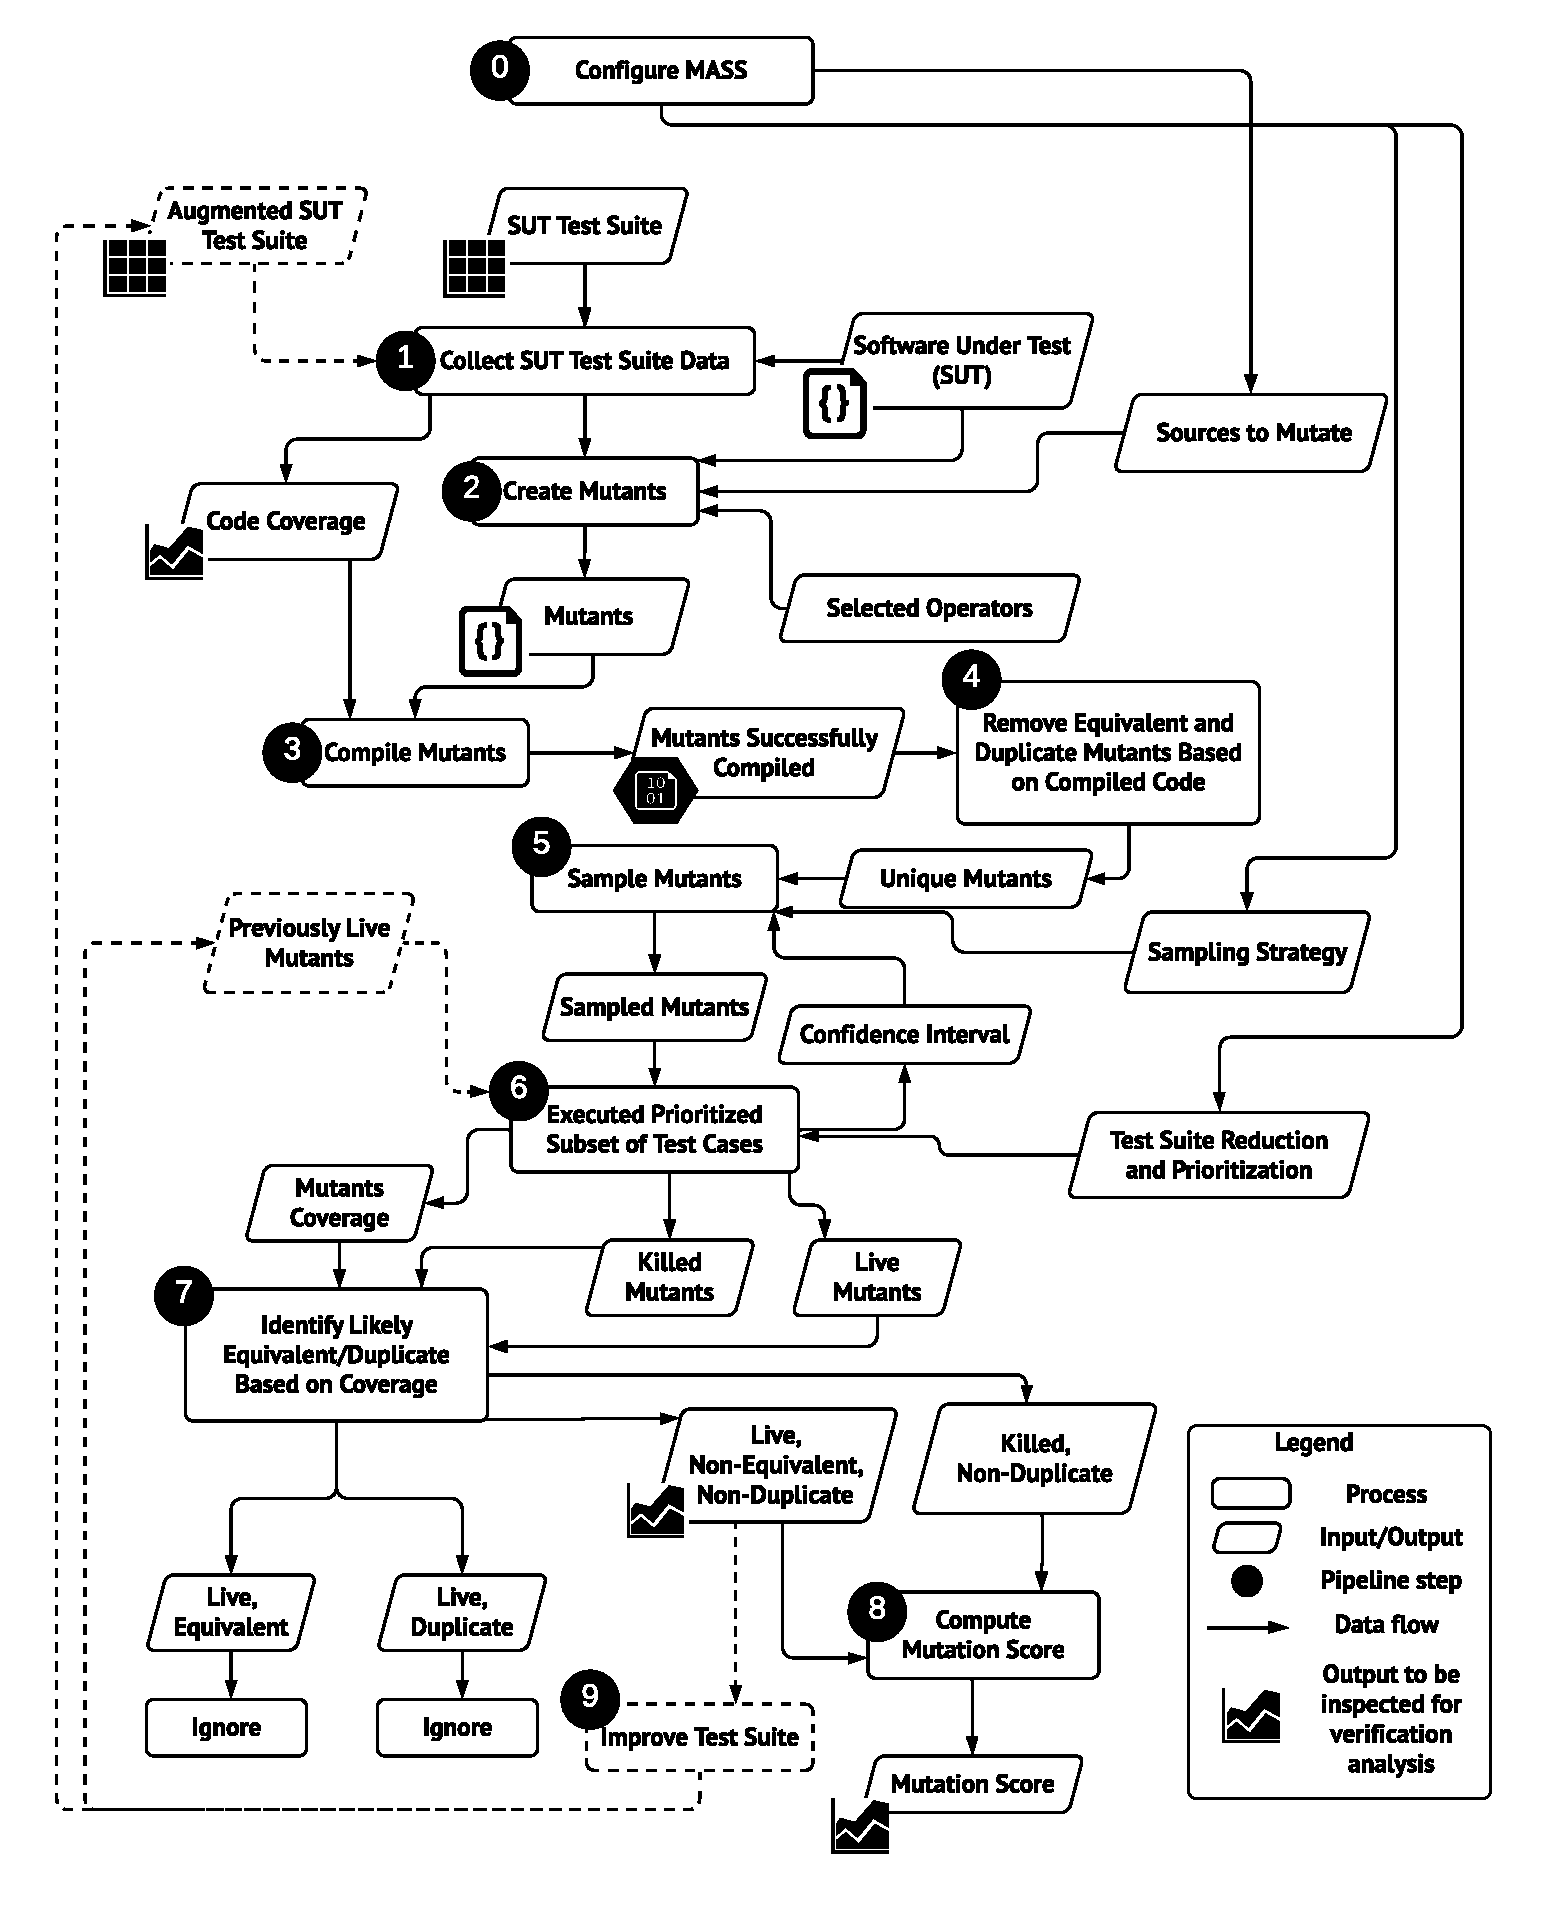
\includegraphics[width=0.8\textwidth]{images/MASS-extended.pdf}
\caption{Overview of the MASS workflow}
\label{fig:MASS}
\end{center}
\end{figure}



The main output of MASS is a file named \emph{MASS\_RESULTS}, which includes the metrics listed in Table~\ref{table:mass:metrics}.
Three additional relevant output files generated by MASS are \emph{filtered\_live}, \emph{useful\_list\_a} and \emph{useful\_list\_b}. They contain the names of the live mutants (i.e., the ones not killed by the test suite), they match the output box \emph{Live, Non-Equivalent, Non-Duplicate} in Figure~\ref{fig:MASS}.

\begin{table}[h]
\caption{MASS Metrics}
\label{table:mass:metrics}
\center
\begin{tabular}{|
@{\hspace{1pt}}p{120mm}|
}
\hline
\textbf{Metric name}\\
\hline
Number of mutants generated \\
%Mutants generation time&No\\
%Number of compiled mutants&No\\
%Percentage of compiled mutants&No\\
%Mutants compilation time&No\\
Number of mutants filtered using compiler optimisations \\
Sampling type \\
Number of mutants executed \\
%Number of test cases executed&No\\
%Test cases execution time \\
%Mutation execution traces \\
Number of killed mutants \\
Number of live mutants \\
Number of likely equivalent mutants \\
MASS mutation score \\
%List of useful mutants \\
Number of statements covered \\
Statement coverage \\
Minimum lines covered per source file \\
Maximum lines covered per source file \\
%Distribution of test cases exercising each statement&No\\
\hline
\end{tabular}
\end{table}

Within file \emph{MASS\_RESULTS}, the \EMPH{first metric} to be inspected is the \emph{Statement coverage} (i.e., the percentage of statements being covered). Since MASS generates mutants only for the statements being exercised by the test suite, a high mutation score in the presence of a low statement coverage cannot indicate that the test suite has high quality. In general, we assume that engineers apply MASS to test suites that have already achieved the required quality level, according to ECSS practice (e.g., statement coverage of 100\%). The statement coverage shall thus simply enable engineers to determine if the test suite is correctly executed through MASS (i.e., if the statement coverage generated by MASS matches the expected one). The statement coverage metric is also generated at the beginning of the mutation analysis process (i.e., Step 1 in Figure~\ref{fig:MASS}\footnote{Statement coverage information is provided in file \emph{coverage.txt.overall}.}); for this reason, in the case of low statement coverage, engineers can focus on improving the test suite without running the rest of the mutation analysis process. The \EMPH{second metric} to be inspected is the \emph{MASS mutation score}. It provides an indication of the quality of the test suite based on mutation analysis results. According to the literature on the topic,
%it shall be above 75\%, otherwise the test suite shall be improved by introducing additional test cases.
 achieving a high mutation score improves significantly the fault detection capability of a test suite~\cite{papadakis2018mutation}; also, a very high mutation score (i.e., above 0.75) ensures a higher fault detection rate than the one obtained with other coverage criteria, such as statement and branch coverage~\cite{Chekam:17}.


\STARTCHANGEDFINAL

An example of the \emph{MASS\_RESULTS} report is presented in Listing~\ref{mass_output}. The output corresponds to mutation analysis process applied to the \emph{MLFS}.

\begin{lstlisting}[language=bash, label=mass_output, caption=\MASS output.]
##### MASS Output #####
## Total mutants generated: 28071
## Total mutants filtered by TCE: 6918
## Sampling type: fsci
## Total mutants analyzed: 461
## Total killed mutants: 369
## Total live mutants: 92
## Total likely equivalent mutants: 53
## MASS mutation score (%): 90.44
## List A of useful undetected mutants: /opt/MLFS/RESULTS/useful_list_a
## List B of useful undetected mutants: /opt/MLFS/RESULTS/useful_list_b
## Number of statements covered: 1973
## Statement coverage (%): 100
## Minimum lines covered per source file: 2
## Maximum lines covered per source file: 138
\end{lstlisting}

The \emph{MASS\_RESULTS} report presented in Listing~\ref{mass_output} contains the following information: total mutants generated (line 3), total mutants filtered by compiler optimisations (line 4), used sampling type (line 5), total mutants analyzed (line 6), total killed mutants (line 7), total live mutants (line 8), total likely equivalent mutants (line 9), MASS mutation score (line 10), list A of useful live mutants (line 11), list B of useful live mutants (line 12), number of statements covered (line 13), statement coverage (line 14), minimum lines covered per source file (line 15), maximum lines covered per source file (line 16).
\ENDCHANGEDFINAL

The next step is the \EMPH{improvement of the test suite}. This is performed by deriving test inputs that kill live mutants.
To this end, engineers shall inspect all the mutants appearing in the file \emph{useful\_list\_a}. For each mutant, the engineer shall implement a test case capable of killing the mutant (i.e., a test case that fails with the mutant but not with the original software).
The file \emph{useful\_list\_a} provides a list of mutants that are likely non redundant with each other because when tested by the SUT test suite they lead to a statement coverage profile (i.e., the set of statements covered during their execution) that differs.
The file \emph{useful\_list\_b} provides a list of mutants that are likely redundant with the ones appearing in the file \emph{useful\_list\_a}; therefore the mutants listed in the file \emph{useful\_list\_b} will be likely killed by test cases implemented to kill the mutants in \emph{useful\_list\_a}.
The mutants within file \emph{useful\_list\_a} are sorted according to their diversity (i.e., the mutants on top are likely very different from each other.
The file \emph{filtered\_live} provides the whole list of live mutants, that is the union of the mutants appearing in the files
\emph{useful\_list\_a} and \emph{useful\_list\_b}.

In general, since a same test case may kill more than one mutant, we suggest to derive test inputs for a subset of the mutants in \emph{useful\_list\_a} and then rerun the mutation analysis process. When rerunning the mutation analysis process, engineers shall focus the mutation analysis on the mutants appearing in \emph{useful\_list\_a} and in \emph{useful\_list\_b}. This is done by re-executing mutation analysis from step 6 (\emph{Execute mutants}), after replacing the mutant names in file \texttt{\$MASS\_WORKSPACE/COMPILED/all\_filtered} by the mutant names of list \emph{useful\_list\_a} and \emph{useful\_list\_b}.

When automated test generation with SEMuS is feasible; we suggest to rely on SEMuS to automatically generate test cases for all the mutants appearing in \emph{useful\_list\_a} and in \emph{useful\_list\_b} (see Section~\ref{sec:meth:semus}).

When identifying inputs that kill mutants (either manually or with SEMuS) engineers may detect equivalent mutants. Equivalent mutants shall be removed from the list of mutants considered for the analysis.

If mutation analysis has been performed through mutants sampling (e.g., with \emph{FSCI}), after test suite improvement (i.e., after introducing test cases that kill all the mutants in \emph{useful\_list\_a} and in \emph{useful\_list\_b}), it is necessary to re-run mutation analysis to estimate the mutation score for the whole system.

\clearpage
\section{Code-driven Mutation Testing: SEMuS}
\label{sec:meth:semus}

Figure~\ref{fig:semus_architecture_meth} provides the workflow of SEMuS; it has been described in Section~\ref{sec:semus}. The list of live mutants processed by SEMuS coincides with the list of mutants appearing in the file \emph{filtered\_live} presented in Section~\ref{sec:meth:mass}.

The mutants for which SEMuS does not generate a test case\footnote{In our toolset, such mutants are identified by looking for empty folders within the output folder \emph{direct/TEMPLATE/FAQAS\_SEMu-out/produced-unittests}.} shall be manually inspected by engineers to determine if they are equivalent to the original software.

The test cases generated by SEMuS can instead be integrated as a regression test suite according to the \EMPH{test suite augmentation} procedure described in Section~\ref{sec:Semus:augment}. Otherwise, engineers can copy the source code of the generated test cases inside the test suite of the SUT and add assertions according to the expected output generated by SEMuS\footnote{Please recall that the output expected after the execution of a test case is written within a file with extension \emph{.expected}, as explained in Section~\ref{sec:Semus:augment}.}.

\begin{figure}[h]
\begin{center}
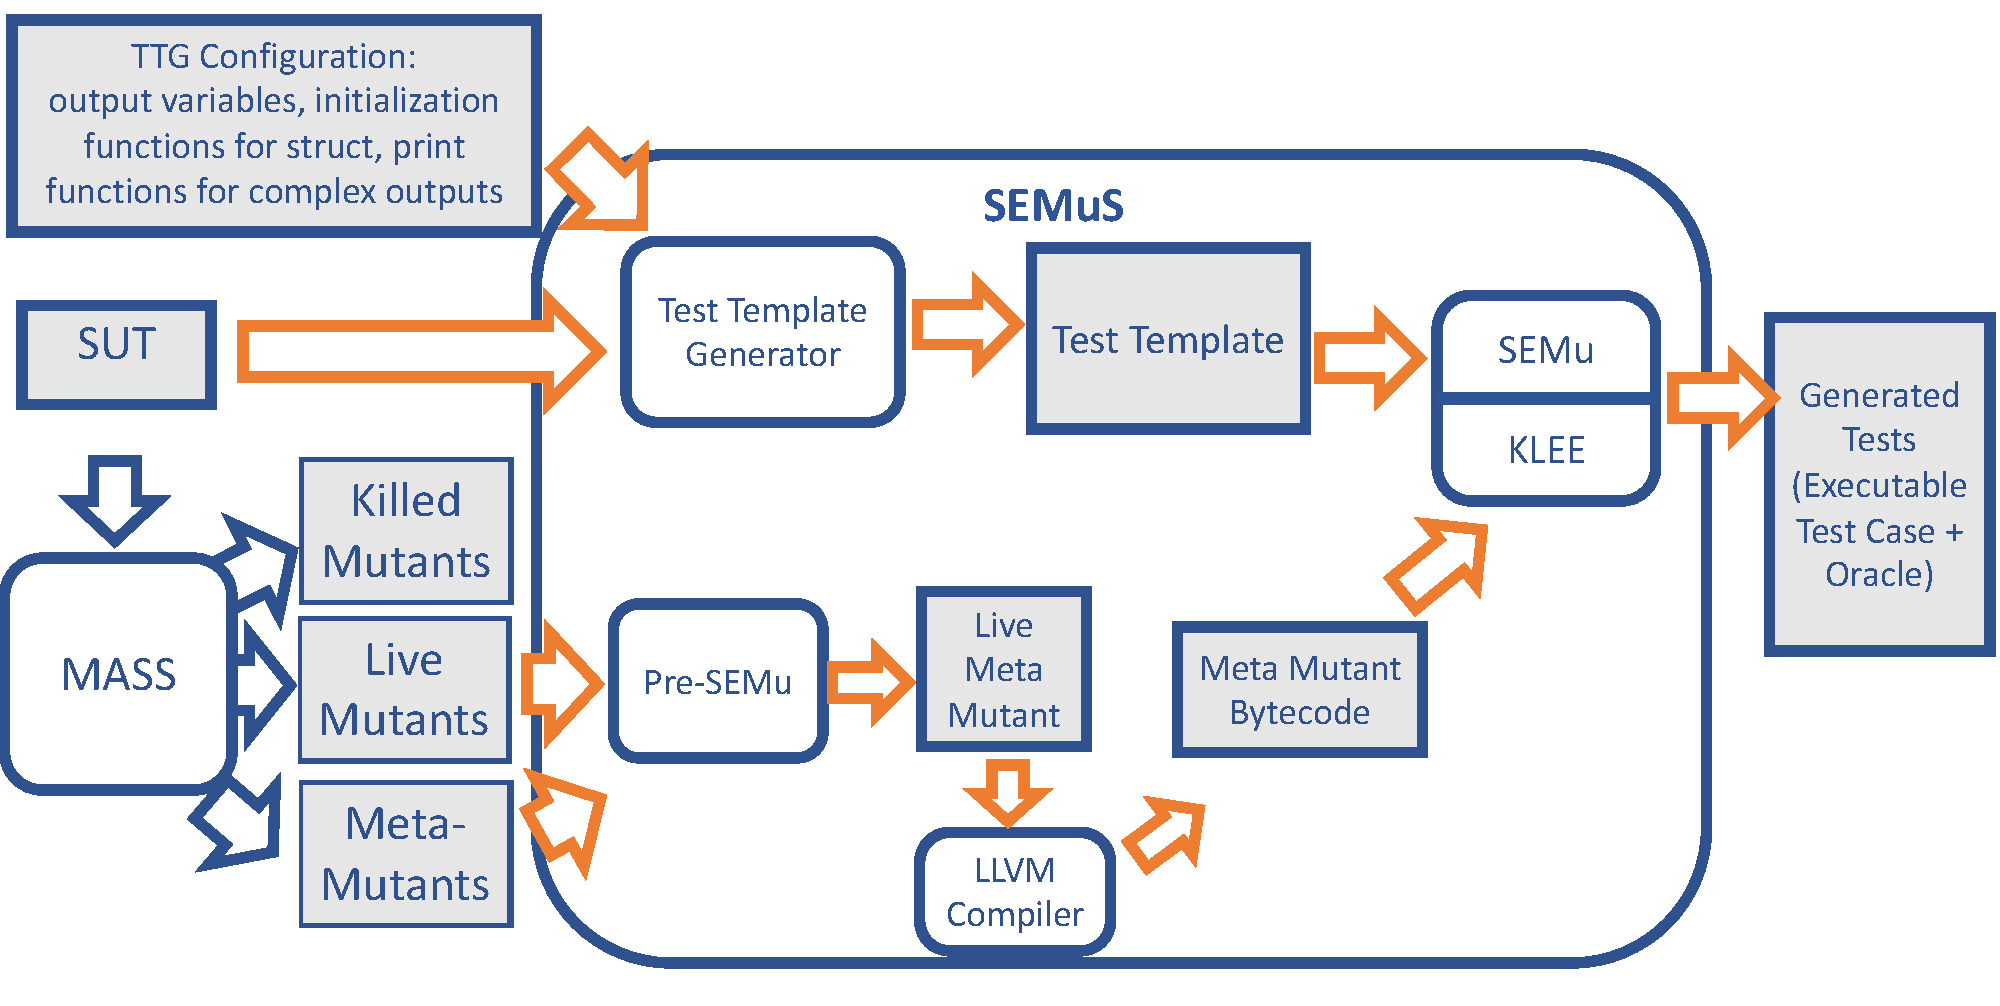
\includegraphics[width=0.8\textwidth]{images/semus-architecture2}
\caption{FAQAS-SEMuS Architecture and Workflow}
\label{fig:semus_architecture_meth}
\end{center}
\end{figure}

\STARTCHANGEDFINAL

The main output of SEMuS is a report file named \emph{AnalysisReport.csv}, which includes the metrics listed in Table~\ref{table:semus:metrics}. These metrics help the SUT engineer to understand at a high level, from the set of live mutants provided to the tool, the number of mutants that were killed by SEMuS (i.e., the tool has generated an input that kills the mutant), the number of mutants that were not killed by SEMuS (i.e., the tool could not generate an input to kill a mutant), and a list showing the status of each mutant (i.e., killed or live).

\begin{table}[h]
\caption{SEMuS Metrics}
\label{table:semus:metrics}
\center
\begin{tabular}{|
@{\hspace{1pt}}p{120mm}|
}
\hline
\textbf{Metric name}\\
\hline
Number of mutants analyzed \\
Number of killed mutants\\
Number of live mutants\\
Mutant statuses\\
\hline
\end{tabular}
\end{table}

An example of the \emph{AnalysisReport.csv} is presented in Listing~\ref{semus_output}.

\begin{lstlisting}[language=bash, label=semus_output, caption=SEMuS output.]
Number of analyzed mutants: 20
Number of killed mutants: 2
Number of live mutants: 18
test.mut.2489.1_1_2.SDL.T_POS_SET_Encode.c;KILLED
test.mut.2489.2_1_14.ICR.T_POS_SET_Encode.c;LIVE
test.mut.2489.1_2_14.ICR.T_POS_SET_Encode.c;LIVE
test.mut.2490.4_1_74.LVR.T_POS_SET_Encode.c;LIVE
test.mut.2491.2_1_10.LCR.T_POS_SET_Encode.c;LIVE
test.mut.2491.2_2_10.LOD.T_POS_SET_Encode.c;LIVE
test.mut.2491.1_1_6.LOD.T_POS_SET_Encode.c;LIVE
test.mut.2491.2_5_23.ROR.T_POS_SET_Encode.c;LIVE
test.mut.2491.4_3_23.ROR.T_POS_SET_Encode.c;LIVE
test.mut.2502.4_8_97.ICR.T_POS_SET_Encode.c;LIVE
test.mut.2502.5_9_97.ICR.T_POS_SET_Encode.c;LIVE
test.mut.2504.2_2_66.LOD.T_POS_SET_Encode.c;LIVE
test.mut.2504.6_1_32.ROR.T_POS_SET_Encode.c;LIVE
test.mut.2506.5_1_96.LVR.T_POS_SET_Encode.c;KILLED
test.mut.2510.5_9_94.ICR.T_POS_SET_Encode.c;LIVE
test.mut.2510.4_8_94.ICR.T_POS_SET_Encode.c;LIVE
test.mut.2512.6_1_36.ROR.T_POS_SET_Encode.c;LIVE
test.mut.2518.5_1_86.LVR.T_POS_SET_Encode.c;LIVE
test.mut.2521.5_1_90.LVR.T_POS_SET_Encode.c;LIVE
test.mut.2524.5_1_98.LVR.T_POS_SET_Encode.c;LIVE
\end{lstlisting}


\section{Code-driven Mutation Testing: Verification Report}


The \emph{Verification Report} is a document that reports on the assessment of a SUT test suite, the analysis shall be based on the FAQAS code-driven mutation testing methodology performed via MASS and SEMuS.

In a nutshell, the report shall provide (1) an introduction to the document, (2) the configuration used to setup the toolset with the SUT, (3) the results of the code-driven mutation analysis process, (4) information about the test cases generated based on mutation testing, and (5) the set of mutants not killed by the approach. More details about the content of the verification report are presented below.

\subsection{Introduction}

This section shall briefly introduce the scope of the verification report and briefly provide essential information on its context and motivation.
It shall contain the following sections:
\begin{enumerate}
    \item \emph{Executive Summary}

    This section shall contain a brief description of the document and a recount of the action taken during the described verification procedure

    \item \emph{ Terms, definitions, and abbreviated terms}

    This section shall contain all the relevant terms, abbreviations and definition used in the documents shall be explained in this section.
\end{enumerate}


\subsection{Configuration of the FAQAS Toolset}

This section shall contain for each tool (i.e., MASS and SEMuS) the specific configurations used to setup the toolset against the SUT. Note that only additional configurations not listed in the software user manual (SUM) document shall be listed (e.g., modifying the optimizations levels for compiler optimisations in MASS, or modifying the test generation time limit in SEMuS).

\subsection{Mutation Analysis Results}

This section shall contain the outcome of the mutation analysis process through the use of MASS. It shall contain the following sections:

\begin{enumerate}
    \item \emph{Source files to be analyzed}

    This section shall contain a subsection specifying the components of the SUT to be considered for the analysis.

    \item \emph{Code coverage}

    This section shall describe the code coverage of the SUT test suite in terms of statement, function, and branch coverage. An action item shall be reported whether the statement or branch coverage does not reach 100\%.

    \item \emph{MASS output}

    It also shall contain a section reporting the outcome of MASS, that is reporting the following metrics:
    \begin{itemize}
        \item The total number of mutants generated, specifying the set of mutation operators used.
        \item The total number of mutants discarded by trivial compiler optimisations.
        \item The total number of mutants tested by MASS.
        \item The total execution time of MASS.
        \item The total number of killed mutants.
        \item The total number of live mutants.
        \item The total number of likely equivalent mutants.
        \item The MASS mutation score.
        \item The statement coverage reached by the test suite.
        \item The total number of statements covered.
        \item The minimum and the maximum number of statements covered per source file.
    \end{itemize}


    \item \emph{Live mutants}

    To finalize, the mutation analysis results shall report a list of five live mutants, that present a behavior that largely differs from that of the original software (i.e., mutants that should have been discovered by the test suite). For each mutant, it shall be reported (1) the source file affected by the mutation, (2) the mutant ID, (3) the excerpt of the function affected by the mutation containing the original version of the software, (4) the excerpt of the function affected by the mutation containing the mutated version of the software, and (5) an action item explaining the problem of the test suite regarding the live mutant.
\end{enumerate}





\subsection{Test Suite Augmentation Results}

This section shall report the outcome of the test suite augmentation process based on mutation testing with SEMuS. This section shall contain the following subsections:

\begin{enumerate}
    \item \emph{Source files to be analyzed}

    This subsection shall list (1) eventual non-processable source files by SEMuS (e.g., source files processing I/O operations, source files with external dependencies), and (2) source files processable by SEMuS.

    \item \emph{SEMuS output}

    The subsection also shall contain a subsection detailing the following test generation metrics:
    \begin{itemize}
        \item The total number of non-processable by SEMuS.
        \item The total number of analyzed mutants by SEMuS.
        \item The total number of additionally killed mutants.
        \item The total number of mutants that are determined by MASS as likely equivalent and for which SEMuS did not generate a test inputs killing them.
        \item The total number of mutants to be manually analyzed by SUT engineers, that is, the set of mutants for which SEMuS was not able to generate a test input for them but MASS did not report them as likely equivalent.
        \item The total number of mutants that reached a test generation timeout during SEMuS analysis.
        \item The updated mutation score including the additionally killed mutants by SEMuS.
    \end{itemize}

    Furthermore, this subsection shall include the list of mutant IDs for the likely equivalent mutants, and for the mutants to be analyzed manually.
\end{enumerate}



\subsection{Software Defects (Optional)}

This section shall report all the software defects spotted by the mutation testing process. For each software defect, the verification report shall specify the (1) inputs generated by SEMuS, (2) the output produced by the SUT with the SEMuS generated inputs, and (3) a brief explanation of the detected software defect.
An action item indicating how to fix the software defect shall be provided to the SUT engineers.

\subsection{Test Cases Generated by SEMuS}

This section shall report the test cases generated by SEMuS. Particularly, for each test case reported, it also shall contain the output produced by the test case. Note that such output can be used as oracle for regression testing (i.e., can be used to verify that updated version of the software still produce the same output).
This section shall be provided as an appendix.


 \ENDCHANGEDFINAL


\clearpage
\section{Data-driven Mutation Analysis: DAMAt}
\label{sec:meth:damat}

DAMAt shall be configured and applied following the procedures described in Section~\ref{sec:damat}.

\STARTCHANGEDFINAL

The primary input for the DAMAt procedure is the fault model.
The fault model is a \texttt{.csv} file, which must be written be the user.
An example of the contents of the fault model file is provided in Listing~\ref{lst:fault_model_meth}

\begin{lstlisting}[caption={Example of a DAMAt fault model, represented in a \texttt{.csv} file. },label={lst:fault_model_meth}]
FaultModel,DataItem,Span,Type,FaultClass,Min,Max,Threshold,Delta,State,Value
GET,6,1,LONG,SS,NA,NA,NA,1,NA,NA
GET,6,1,LONG,SS,NA,NA,NA,-1,NA,NA
SET,6,1,BIN,BF,0,7,NA,NA,-1,1
SAVE,6,1,LONG,SS,NA,NA,NA,1,NA,NA
SAVE,6,1,LONG,SS,NA,NA,NA,-1,NA,NA
SAVE,7,1,LONG,SS,NA,NA,NA,1,NA,NA
SAVE,7,1,LONG,SS,NA,NA,NA,-1,NA,NA
LOAD,6,1,LONG,SS,NA,NA,NA,1,NA,NA
LOAD,6,1,LONG,SS,NA,NA,NA,-1,NA,NA
LOAD,7,1,LONG,SS,NA,NA,NA,1,NA,NA
LOAD,7,1,LONG,SS,NA,NA,NA,-1,NA,NA
REPLY,2,1,LONG,SS,NA,NA,NA,1,NA,NA
REPLY,2,1,LONG,SS,NA,NA,NA,-1,NA,NA
REPLY,2,1,LONG,IV,NA,NA,NA,NA,NA,0
REPLY,2,1,LONG,VAT,NA,NA,180,1,NA,NA
REPLY,2,1,LONG,FVAT,NA,NA,180,1,NA,NA
REPLY,4,1,LONG,SS,NA,NA,NA,1,NA,NA
REPLY,4,1,LONG,SS,NA,NA,NA,-1,NA,NA
REPLY,5,1,LONG,SS,NA,NA,NA,1,NA,NA
REPLY,5,1,LONG,SS,NA,NA,NA,-1,NA,NA
REPLY,6,1,BIN,BF,0,7,NA,NA,-1,1
\end{lstlisting}

Every line of the file represents a mutation operator, while every column represents a configuration parameter for that operator.

\begin{itemize}
  \item Column \emph{FaultModel} contains the name of the Fault Model containing the operator. Typically the user shall define a fault model for every different kind of message exchanged through the buffer.

  \item Column \emph{DataItem} refers to the index of the first element of the targeted data item in the array representing the buffer.

  \item Column \emph{Span} reports the number of array elements that make up the data item target by the mutation.

  \item Column \emph{Type} reports about the type of data targeted by the mutation: \texttt{INT}, \texttt{LONG}, \texttt{FLOAT}, \texttt{DOUBLE}, \texttt{BIN} or \texttt{HEX}.

  \item Column \emph{FaultClass} contains the type of fault that the mutation will emulate.

  \item The other columns represent configuration parameters and assume different meanings depending on the mutation operator they refer to. More details on the data-driven mutation operators and their configuration can be found in Section~\ref{sec:damat}.
\end{itemize}

There are some other variables that influence the behaviour of the DAMAt tool.
They are contained in the file \texttt{DAMAt\_configure.sh}. The value of these variable shall be set by the user.

\begin{itemize}
  \item The variable \texttt{fault\_model} shall be set to the path of the csv containing the fault model of the Software Under Test defined by the engineer.
  This will allow the tool to generate the mutation API starting from the correct fault model.
  \item The variable \texttt{buffer\_type} shall contain the type of the elements of the buffer that will be targeted by the mutation (i.e. \texttt{int}, \texttt{float}, \texttt{double} etc.).
  \item The variable \texttt{singleton} shall be set to \texttt{TRUE} or \texttt{FALSE}. If set to \texttt{TRUE}, the Fault Model will be initialized in a singleton variable, to avoid memory issues.
  \item The variable \texttt{padding} shall be set to an integer number representing the number of bytes to skip at the beginning of the target buffer. Normally it shall be set to \texttt{0}, but it can be used to skip the header of the buffer if needed.
\end{itemize}

The DAMAt pipeline can then be executed. The DAMAt toolset will automatically generate the mutants and execute the generated mutants against the test suite under evaluation.
Every mutation operator can will generate one or more mutants.

\ENDCHANGEDFINAL


% DAMAt shall be configured and applied according to the procedure described in Section~\ref{sec:damat}.
After the execution, DAMAt generates two files: \emph{final\_mutants\_table.csv} and \emph{mutation\_sum\_up.csv}.
The latter provides a high-level perspective on the results of the procedure, because it contains the three metrics defined in Section~\ref{sec:mutationAnalysisResults}:
\begin{enumerate}
\item Fault model coverage, the percentage of fault models covered by the test suite.
\item Mutation operation coverage, the percentage of data items that have been mutated at least once, considering only those that belong to the data buffers covered by the test suite.
\item Mutation Score, the percentage of mutants killed by the test suite (i.e., leading to at least one test case failure) among the mutants that target a fault model and for which at least one mutation operation was successfully performed.
\end{enumerate}


A low score in one of the metrics indicate one of following scenarios, respectively:
\begin{enumerate}
\item The message type targeted by a fault model is never exercised.
\item The message type is covered by the test suite, but it is not possible to perform some of the mutation operations. It depends on the fact that not all the input partitions are exercised by the test suite.
\item The mutation is performed but the test suite does not fail. It may depend on two reasons: (1) the test oracles are imprecise (e.g., they do not verify all the state variables), (2) the system is not brought into a state where the effect of the mutation is notices (i.e., the scenarios exercised are insufficient).
\end{enumerate}

\STARTCHANGEDFINAL

On the other hand, \emph{final\_mutants\_table.csv}, contains a list of all generated mutants, the definition of the mutation operator that generated them and their status. It can be useful to determine how to improve the test suite.

An example of \emph{final\_mutants\_table.csv} is represented in Figure~\ref{fig:damat:example:result:table}.

 \begin{figure}[h]
\begin{center}
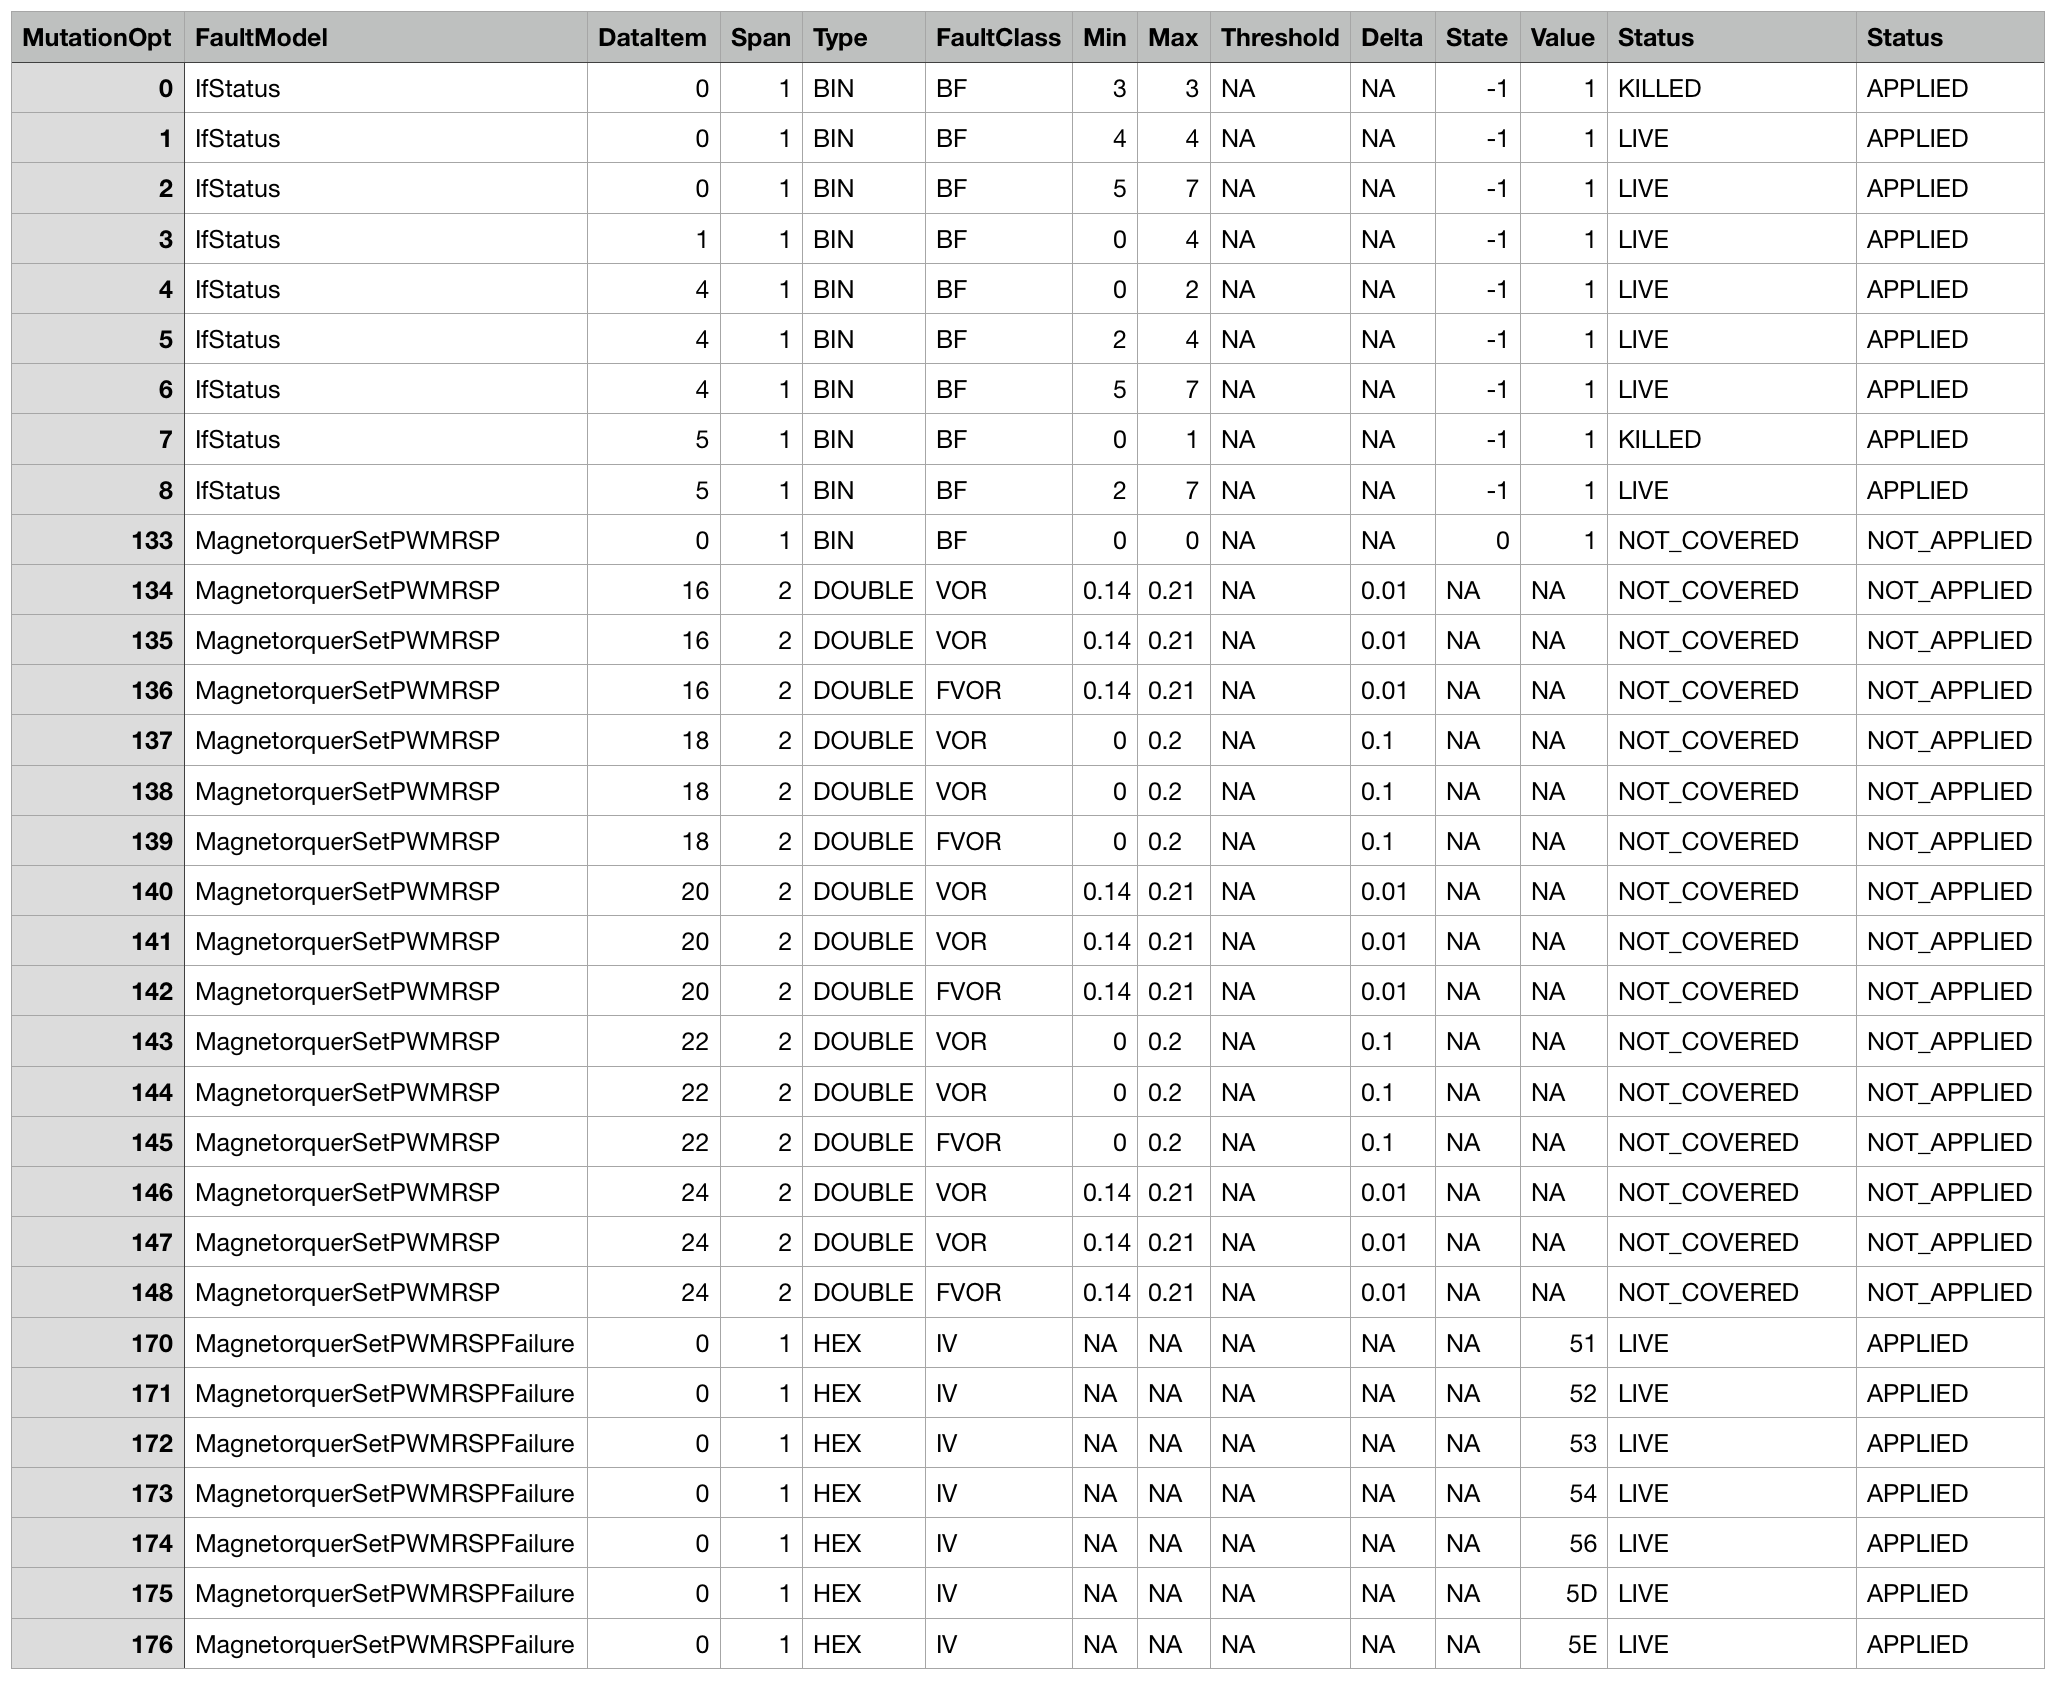
\includegraphics[width=0.8\textwidth]{images/DAMAtADCS.png}
\caption{DAMAt: Example of the result table \emph{final\_mutants\_table.csv}.}
\label{fig:damat:example:result:table}
\end{center}
\end{figure}

Every line in the table represents a different mutant.

Column \emph{MutationOpt} contains a unique numerical identifier for each mutant.

The columns from \emph{FaultModel} to \emph{Value} contain the definition of the mutation operator that generated the mutant.

\ENDCHANGEDFINAL

Column \emph{Status} reports about  the fault model coverage; indeed, mutants reported as \emph{NOT\_COVERED} indicate that the corresponding fault model is not covered by the test suite. Since we define a different fault model for each type of message exchanged by the software under test (e.g., each message may correspond to a different PUS command), the lack of coverage for a fault model indicates that a message type has not been exercised at all by the test suite. In practice this also means that the line of code where the mutation probe has been placed was not exercised.
To address such shortcoming, the the engineer shall define a test case that makes the SUT send that particular message type (or receive that particular message type).

The column named \emph{application} reports about the \emph{mutation operation coverage}. By looking at the mutants defined as \emph{NOT\_APPLIED} the engineer can determine if some input partitions (i.e., some subsets of the input range) had not been exercised by the test suite. Table~\ref{table:damat:interpretation} describes how to interpret the result reported in the Application column, for each type of mutant.
For example, if there is a Value Above Threshold that is not applied, this means that the particular data item targeted by the mutation was never below that threshold during the test suite execution.
This could give an insight on what kind of data is exchanged by the components during the execution to help determine if some use case is not considered in the test suite.


Last, by looking at what mutants remain LIVE after the execution of DAMAt, the user can identify cases in which the test suite does not fail although the data being exchanged is not the one expected by the engineer who wrote the test suite.
The simplest cause of such lack of failures is the absence of an oracle (or a poor oracle); for example, the test case assertions do not verify the output state of the SUT.
Another possibility is that the software reacts to the invalid data only when in a specific state; this means that the test suite lacks a test case in such a specific state.

For DAMAt, \EMPH{test suite augmentation} shall thus be performed manually by an engineer who shall define additional test cases based on the strategy reported above.

% !TEX root = ../MAIN.tex
\begin{table}[H]
\caption{Interpretation of results concerning the lack of coverage for mutation operations.}
\label{table:damat:interpretation}
\begin{tabular}{|p{2cm}|p{6cm}|p{6cm}|}
\hline
\textbf{Mutation Operator} & \textbf{If APPLIED} & \textbf{If NOT\_APPLIED} \\ \hline
\textbf{VAT} & The value of the targeted data item was below the threshold at least once. & The value of the targeted data item was never below the threshold. It indicates that the test suite does not cover the input partition (e.g., the test suite never tests the nominal case). \\ \hline
\textbf{VBT} & The value of the targeted data item was above the threshold at least once. & The value of the targeted data item was never above the threshold. It indicates that the test suite does not cover the input partition (e.g., the test suite never tests the nominal case). \\ \hline
\textbf{VOR} & The value of the targeted data item was inside the range defined by Min and Max at least once. & The value of the targeted data item was never observed within the range defined by Min and Max. It indicates that the test suite does not cover the min-max input partition (e.g., the test suite never tests the nominal case). \\ \hline
\textbf{BF} & At least a bit was flipped. If State was set to 1 this means that between Min and Max position at least a bit contained a 1. The same goes if State was set to 0. & No bits were flipped, this happens when the test suite never lead to the exchange of messages containing bits in the specified state (either $0$ or $1$). It indicates that an input partition is not covered.\\ \hline
\textbf{INV} & It is always applied.& It is always applied.\\ \hline
\textbf{IV} & The value of the targeted data item was different from the invalid value specified by the operator at least once.&
The value of the targeted data item was always equal to the invalid value specified by the operator at least once. It indicates that the test suite only test the software in the presence of a specific invalid value.\\ \hline
\textbf{ASA} & It is always applied.& It is always applied.\\ \hline
\textbf{SS} & It is always applied.& It is always applied.\\ \hline
\textbf{HV} & It is always applied.& It is always applied.\\ \hline
\textbf{FVAT} & The value of the targeted data item was above the threshold at least once. &
The value of the targeted data item was never above the threshold. It indicates that the test suite does not cover the input partition (e.g., it does not cover non-nominal cases).\\ \hline
\textbf{FVBT} & The value of the targeted data item was below the threshold at least once. & The value of the targeted data item was never below the threshold. It indicates that the test suite does not cover the input partition (e.g., it does not cover non-nominal cases).\\ \hline
\textbf{FVOR} & The value of the targeted data item was outside the range defined by Min and Max at least once. & The value of the targeted data item was never outside the range defined by Min and Max. It indicates that the test suite does not cover the input partition (e.g., it does not cover non-nominal cases). \\ \hline
\end{tabular}
\end{table}



\STARTCHANGEDFINAL
\section{Data-driven Mutation Testing: Verification Report}
A verification report written after an execution of \DAMA shall account for all the most relevant results produced during the procedure. We propose the following structure.

  \subsection{Introduction}


  This chapter shall briefly introduce the scope of the verification report and briefly provide essential information on its context and motivation.
  It shall contain the following sections:
  \begin{enumerate}


    \item \emph{Executive Summary}


    This section shall contain a brief description of the document and a recount of the action taken during the described verification procedure.


    \item \emph{Terms, definitions, and abbreviated terms}


    All the relevant terms, abbreviations and definition used in the documents shall be explained in this section.


  \end{enumerate}


  \subsection{Configuration of the Toolset}


  This chapter shall describe how \DAMA was configured for the particular use case for which the procedure has been performed.
  It shall contain the following sections:
  \begin{enumerate}


    \item \emph{Probe Insertion Strategy}


    This section shall describe and motivate where and how the mutation probes were placed in the source code. It shall briefly explain the reasoning behind choosing the target file and function and highlight any particularity of the probe insertion (i.e. additional lines of code etc.).


    \item \emph{Fault Model}


    This section shall describe the composition of the Fault Model, report it in tabular form and briefly explain what were the type of message that were targeted. It should also contain a brief explanation on how to read the fault model itself (i.e. meaning of the columns) and a table containing the definitions of the mutation operators.


  \end{enumerate}


  \subsection{Results}


  This chapter shall describe the results of the \DAMA procedure. A brief introduction shall report the \emph{FMC}, \emph{MOC} and \emph{MS} metrics, and explain their meaning in the context of \DAMA.
  Then different section will address the limitation of the test suite as indicated by the metrics and suggest addiction item to improve it.
  It shall contain the following sections as needed:
  \begin{enumerate}


    \item \emph{Fault Model Coverage (optional)}


    If the \emph{Fault Model Coverage (optional)} is below 100\%, this section will report which mutation probes were not covered by the test suite and their placement in the code. The suggested action item shall be devising test that cover the branches in question.


    \item \emph{Mutation Operation Coverage (optional)}


    If the \emph{Mutation Operation Coverage} is below 100\%, this section will report the number of mutants covered but not applied and their definition.
    For everyone of these mutants, the suggested action item shall be to check why the input partition related to that mutant is not covered and why.


    \item \emph{Mutation Score (optional)}


    If the \emph{Mutation Score} is below 100\%, this section will report the number of mutants applied but not killed and their definition.
    For everyone of these mutants, the suggested action item shall be to check if an oracle for that data item exists and, in that case, if it is well defined.


  \end{enumerate}

\ENDCHANGEDFINAL
